%%
% The SUEPThesis Template for Bachelor Graduation Thesis
%
% 上海电力大学毕业设计(论文)中英文摘要 —— 使用 XeLaTeX 编译
%
% Copyright 2020-2023 SUEPaper
%
% This work may be distributed and/or modified under the
% conditions of the LaTeX Project Public License, either version 1.3
% of this license or (at your option) any later version.
% The latest version of this license is in
%   http://www.latex-project.org/lppl.txt
% and version 1.3 or later is part of all distributions of LaTeX
% version 2005/12/01 or later.
%
% This work has the LPPL maintenance status `maintained'.
%
% The Current Maintainer of this work is Haiwen Zhang.
%%

\chapter{考虑检修的WPCR生产和存储模型}

\section{考虑检修的生产和存储模型建立}

为了保障生产的持续性,工厂需要在30周210天里必须设置7次停工检修,每次检修时间为1天。
检修后的第一天A、B、C生产总工时限制将会放宽10\%,随后逐日减少放宽2\%的比例,
直至为0。设衰减系数为$\lambda$
\begin{equation}
    \lambda (k)=0.1-\lambda \cdot (k-1)
\end{equation}
\begin{equation}
    k \leq 6
\end{equation}

设检修当天为第$d$天
\begin{equation}
    T_d=0,x_d=0
\end{equation}
\begin{equation}
    d(0)=d
\end{equation}
\begin{equation}
    d(k)=d(k-1)+k \qquad k=1,2,...,6
\end{equation}
\begin{equation}
    T_{d(k)}=T_{d(k)}\cdot [1+\lambda(k)]
\end{equation}

最后求解同理连续多周生产统筹规划模型。
\begin{equation}
    \min\sum_{k=1}^{n}(
            C_{\uppercase\expandafter{\romannumeral1}}^{'''}+
            C_{\uppercase\expandafter{\romannumeral2}}^{'''}+
            C_{\uppercase\expandafter{\romannumeral3}}^{'''}) 
\end{equation}

\section{考虑检修的生产和存储模型求解}

\subsection{考虑检修的生产和存储模型求解算法}
遗传算法\cite{王小平2002遗传算法}是一种全局最小费用优化方法,并且已经有研究表明多变量编码遗传算法
\cite{张京京2022多变量编码遗传算法在管道类零件展开图排样中的应用,jiyugaijinyichuansuanfa}
能够准确地表征排样件的几何形状及位置特征,保证了高效率排样,提高了排样的材料利用率,
同时,验证了多变量编码遗传算法具有可行性与有效性,对于优化钣金件制造加工工艺、
提高生产效率具有重要指导意义。因此在本模型中可以采用遗传环境适应的方法得到最优结果,
遗传算法实现包括以下步骤:

S1:染色体编码;

S2:种群初始化;

S3:计算适应度函数;

S4:选择;

S5:交叉;

S6:变异;

S7:进化逆转 ;

S8:对随机初值进行优化,并得到新种群;

S9:判断是否达到最大遗传代数,若是则输出结果;若不是,则返回S3。

遗传算法流程图如图\ref{f.ch4-1}所示:

\begin{figure}[h]
    \centering
    \begin{tikzpicture}[node distance=25pt]
    \node[draw, rounded corners]                        (start)   {待优化的问题};
    \node[draw, below=of start]                         (step 1)  {确定目标函数和解的空间};
    \node[draw, below=of step 1]                        (step 2)  {计算个体的适应度值};
    \node[draw, diamond, aspect=2, below=of step 2]     (choice)  {满足收敛条件或达到进化代数};
    \node[draw, right=30pt of choice]                   (step x)  {遗传算子操作生成新种群};
    \node[draw, rounded corners, below=20pt of choice]  (end)     {输出最优解};
    
    \draw[->] (start)  -- (step 1);
    \draw[->] (step 1) -- (step 2);
    \draw[->] (step 2) -- (choice);
    \draw[->] (choice) -- node[left]  {是} (end);
    \draw[->] (choice) -- node[above] {否}  (step x);
    \draw[->] (step x) -- (step x|-step 2) -> (step 2);
\end{tikzpicture}
    \caption{遗传算法流程图}
    \label{f.ch4-1}
\end{figure}

Step1:采用整数排列的编码方法,随机生成由$1~n$个整数构成的染色体,
每个整数基因对应n个生产需求点;每条染色体可划分为几个不同的部分,
每个部分即不同检修点的集合;各基因的排列顺序决定对应检修点的排列顺序,
从随机初始位置开始,按排列顺序依次将各检修节点加入到整个30周的组装计划中,
每加入一个检修节点,计算是否满足约束条件,未超出条件,
则继续加入下一检修节点,直到超出约束范围,则进入本初始条件下的顺序分配;
重复分配$k$次,得到所有检修节点的组合,将每次获得的检修节点顺序结合,
即总的生产组装安排计划\cite{包子阳2016智能优化算法}。

Step2:染色体编码完成后,生成一个包含若干条染色体的初始种群;
计算适应度函数,以最小化费用为目标,适应度值取目标函数的倒数,
计算过程如下:
\begin{equation}
    \label{eq_fitness}
    fitness=\frac{1}{z}
\end{equation}

选择是从一个旧种群中选择生命力强的个体位串,产生新种群的过程。
本例中选择操作采用适度比例法,它根据某个体的适应度与该代全部个体适应度之和的比值,
来决定其子孙遗留的可能性,即在第$n$代中,某个体$i$被选取的概率为:
\begin{equation}
    P_{si}=\frac{f_i}{\sum f_N}
\end{equation}

其中,$f_i$为某个体的适应度,$\sum f_N$为该代全部个体的适应度之和,可根据式\ref{eq_fitness}来进行计算。
确定概率后,可用轮盘赌的选择方法来实现选择操作。
例如,用计算机生成$0~1$之间均匀分布的随机数,若$P=0.5$,则当产生的随机数在$0~0.5$之间时,该串被复制,否则被淘汰。

Step3:交叉运算是指两个相互配对的染色体按某种方式相互交换某部分基因,从而形成两个新的个体。
在遗传算法中,将种群中的$N$个个体以随机的方式组成$N/2$对配对个体组,
交叉操作在这些配对个体组中的两个个体间进行的。

考察某配对个体组中的两个个体$a$、$b$,交叉操作采用一定方式将它们变为两个新的个体$a^{'}$、$b^{'}$。
在遗传算法中,交叉操作过程需要满足:
\begin{equation}
    a+b=a^{'}+b^{'}
\end{equation}

基于上式,浮点数编码的交叉操作采用如下方式来实现:
\begin{equation}
    \begin{cases}
        a^{'}=(1-\alpha)\alpha+\beta b \\
        b^{'}=(1-\beta)\beta+\alpha a
    \end{cases}
\end{equation}

其中,$\alpha$、$\beta$为区间上均匀分布的随机数,且有$r\leq1$,
调整$r$的大小即可控制交叉操作的变化范围。

Step4:使用变异算子来调整个体编码串中的部分基因值,
可以从局部的角度出发使个体更加逼近最优解,提高遗传算法的局部搜索能力。
变异操作将某个个体的参数$c$,操作变为域内的另一个值$c^{'}$。浮点数编码的遗传算法采用下式进行:
\begin{equation}
    c^{'}=N(c,\sigma)
\end{equation}

其中,$c^{'}=N(c,\sigma)$表示平均值为$c$,方差为$\sigma$的正态分布随机数。可以看出,变异操作即是以当前值为中心,
主要在一个小范围内进行随机扰动的变化\cite{余胜威2015matlab}。

根据连续多周生产统筹规划的WPCR生产和存储模型,结合遗传算法,
求解得到如图\ref{f.ch4-2}所示基于遗传算法的机器人组装计划费用优化。
从图\ref{f.ch4-2}可以看出,随着迭代次数的增多,到达一定迭代次数,最小费用和平均费用都趋于稳定。

\begin{figure}[H]
    \centering
    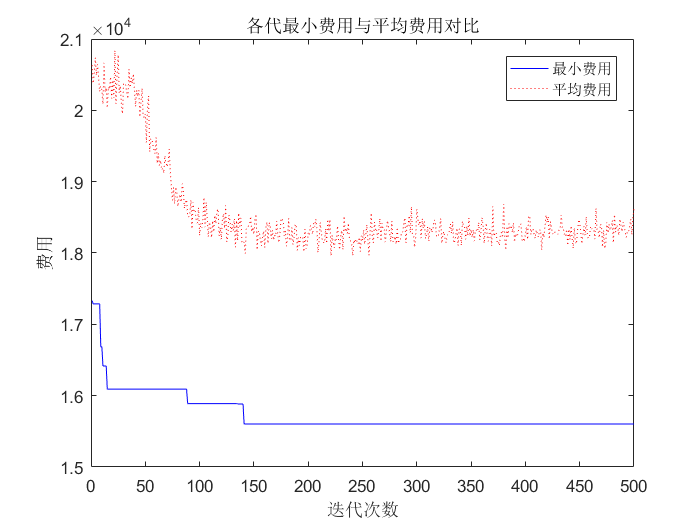
\includegraphics[width=0.7\linewidth]{ch4-2.png}
    \caption{迭代费用对比}
    \label{f.ch4-2}
\end{figure}


\begin{table}[!hpt]
    \caption{考虑检修的生产和存储模型求解的结果}
    \label{T.ch4-1}
    \centering
    \renewcommand\arraystretch{1.5} 
    \begin{tabular}{@{}cccccccc@{}} 
    \toprule
    \textbf{第1次} & \textbf{第2次} & \textbf{第3次} & \textbf{第4次} & \textbf{第5次} & \textbf{第6次} & \textbf{第7次} & \textbf{总成本} \\
    \midrule
    24  & 72 & 99 & 120 & 153 & 171 & 202 & 6308701 \\
    \bottomrule
    \end{tabular}
\end{table}

\begin{longtable}[c]{c*{7}{r}}
    \caption{考虑检修的生产和存储模型求解结果展示}
    \label{T.ch4-2} \\
    \toprule
    \textbf{天} & \textbf{周一} & \textbf{周二} & \textbf{周三} & 
    \textbf{周四} & \textbf{周五} & \textbf{周六} & \textbf{周日} \\
    \midrule
    \endfirsthead
    \multicolumn{8}{l}{\textbf{续表~\thetable}} \\

    \toprule
    \textbf{天} & \textbf{周一} & \textbf{周二} & \textbf{周三} & 
    \textbf{周四} & \textbf{周五} & \textbf{周六} & \textbf{周日} \\
    \midrule
    \endhead
    \hline
    \multicolumn{8}{r}{续下页}
    \endfoot
    \endlastfoot
    \textbf{第1周}  & 1 & 2 & 3 & 4 & 5 & 6 & 7 \\ 
    \textbf{第2周}  & 1 & 2 & 3 & 4 & 5 & 6 & 7 \\ 
    \textbf{第3周}  & 1 & 2 & 3 & 4 & 5 & 6 & 7 \\ 
    \textbf{第4周}  & 1 & 2 & 3 & 4 & 5 & 6 & 7 \\
    \textbf{第5周}  & 1 & 2 & 3 & 4 & 5 & 6 & 7 \\
    \textbf{第6周}  & 1 & 2 & 3 & 4 & 5 & 6 & 7 \\
    \textbf{第7周}  & 1 & 2 & 3 & 4 & 5 & 6 & 7 \\
    \textbf{第8周}  & 1 & 2 & 3 & 4 & 5 & 6 & 7 \\ 
    \textbf{第9周}  & 1 & 2 & 3 & 4 & 5 & 6 & 7 \\ 
    \textbf{第10周}  & 1 & 2 & 3 & 4 & 5 & 6 & 7 \\
    \textbf{第11周}  & 1 & 2 & 3 & 4 & 5 & 6 & 7 \\
    \textbf{第12周}  & 1 & 2 & 3 & 4 & 5 & 6 & 7 \\
    \textbf{第13周}  & 1 & 2 & 3 & 4 & 5 & 6 & 7 \\
    \textbf{第14周}  & 1 & 2 & 3 & 4 & 5 & 6 & 7 \\
    \textbf{第15周}  & 1 & 2 & 3 & 4 & 5 & 6 & 7 \\
    \textbf{第16周}  & 1 & 2 & 3 & 4 & 5 & 6 & 7 \\
    \textbf{第17周}  & 1 & 2 & 3 & 4 & 5 & 6 & 7 \\
    \textbf{第18周}  & 1 & 2 & 3 & 4 & 5 & 6 & 7 \\
    \textbf{第19周}  & 1 & 2 & 3 & 4 & 5 & 6 & 7 \\
    \textbf{第20周}  & 1 & 2 & 3 & 4 & 5 & 6 & 7 \\
    \textbf{第21周}  & 1 & 2 & 3 & 4 & 5 & 6 & 7 \\
    \textbf{第22周}  & 1 & 2 & 3 & 4 & 5 & 6 & 7 \\
    \textbf{第23周}  & 1 & 2 & 3 & 4 & 5 & 6 & 7 \\
    \textbf{第24周}  & 1 & 2 & 3 & 4 & 5 & 6 & 7 \\
    \textbf{第25周}  & 1 & 2 & 3 & 4 & 5 & 6 & 7 \\
    \textbf{第26周}  & 1 & 2 & 3 & 4 & 5 & 6 & 7 \\
    \textbf{第27周}  & 1 & 2 & 3 & 4 & 5 & 6 & 7 \\
    \textbf{第28周}  & 1 & 2 & 3 & 4 & 5 & 6 & 7 \\
    \textbf{第29周}  & 1 & 2 & 3 & 4 & 5 & 6 & 7 \\ 
    \textbf{第30周}  & 1 & 2 & 3 & 4 & 5 & 6 & 7 \\ 
    \bottomrule
\end{longtable}